\documentclass[a4paper,12pt]{article}
\usepackage{tikz}
\usepackage[utf8]{inputenc}
\usepackage[greek,english]{babel}
\usepackage{alphabeta}
\usepackage{amsmath}     % Core AMS math features
\usepackage{amssymb}     % Extended symbol collection
\usepackage{amsthm}      % For theorems and proofs
\usepackage{geometry}
\geometry{a4paper, margin=1in}
\usepackage{setspace}
\usepackage{graphicx}
\usetikzlibrary{shapes.geometric, arrows}
\usetikzlibrary{positioning}
\usepackage{hyperref}
\usepackage{fancyhdr}
\usepackage{datetime2}
\usepackage{xcolor}
\usepackage{kerkis} %ΚΑΛΟΟΟΟ
\usetikzlibrary{arrows.meta}
\usetikzlibrary{shadows}
\usetikzlibrary{backgrounds}


\usepackage{eulervm}



\definecolor{mycolor}{RGB}{241, 237, 221,} % A light yellowish color
\pagecolor{mycolor}


\pagestyle{fancy}  % Enable fancy style
\fancyhf{}  % Clear all header and footer settings



\setstretch{1.2}


\begin{document}


\begin{titlepage}
    \centering
    \vspace*{3cm}
    \hrule \vspace{1cm}
    {\Huge \textbf{Machine Learning (Basics) with numpy} \par}
    {\Large \textbf{} \par}
    \vspace{1cm} \hrule
    
%%%%%%%%%%%%%%%%%%%%%%%%%%%
\vspace{3cm}
\begin{center}
\tikzset{%
  every neuron/.style={
    circle,
    draw,
    minimum size=1cm
  },
  neuron missing/.style={
    draw=none, 
    scale=4,
    text height=0.333cm,
    execute at begin node=\color{black}$\vdots$
  },
}

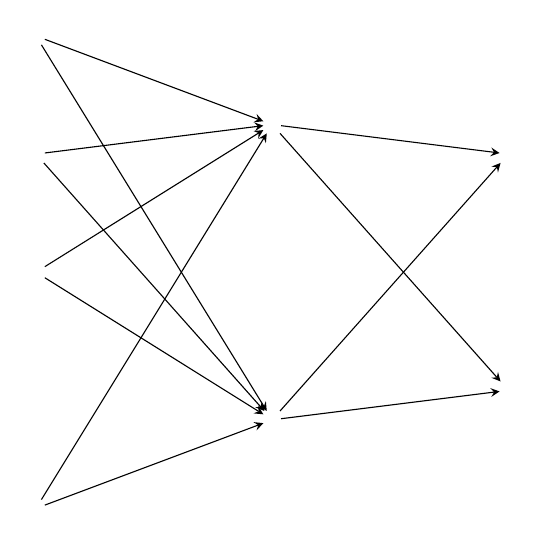
\begin{tikzpicture}[x=1.5cm, y=1.5cm, >=stealth]

% Input layer neurons
\foreach \m/\l [count=\y] in {1,2,3,missing,4}
  \node [every neuron/.try, neuron \m/.try] (input-\m) at (0,2.5-\y) {};

% Hidden layer neurons
\foreach \m [count=\y] in {1,missing,2}
  \node [every neuron/.try, neuron \m/.try ] (hidden-\m) at (2,2-\y*1.25) {};

% Output layer neurons
\foreach \m [count=\y] in {1,missing,2}
  \node [every neuron/.try, neuron \m/.try ] (output-\m) at (4,1.5-\y) {};

% Input to hidden layer connections
\foreach \i in {1,...,4}
  \foreach \j in {1,...,2}
    \draw [->] (input-\i) -- (hidden-\j);

% Hidden to output layer connections
\foreach \i in {1,...,2}
  \foreach \j in {1,...,2}
    \draw [->] (hidden-\i) -- (output-\j);

\end{tikzpicture}
\end{center}

%%%%%%%%%%%%%%%%%%%%%%%%%%%
        \vfill

    {\large Βασίλης Ρουσόπουλος \par}
    %{\large Προπτυχιακός Φοιτητής Μαθηματικού Αθήνας ΕΚΠΑ \par}
    (Documentation του σχετικού προγράμματος αναγνώρισης χειρόγραφων αριθμών)
\end{titlepage}

%%%%%%%%%%%%%%%%%%%%%%%%%%%%%%%%%%%%%%%%%%%%%%%%%%%%%%%%%%%%%%%%%%%%%%%%%%%%

\pagenumbering{roman}
\begin{titlepage} 
    \centering
    \vspace{1cm} 
    \tableofcontents
    \vfill 
\end{titlepage}
\clearpage
\markright{}
% Section name on top right
\fancyhead[R]{\nouppercase{\rightmark}}  

% Page number centered at the bottom
\fancyfoot[C]{\thepage}  

% Ensure section names update correctly
\renewcommand{\sectionmark}[1]{\markright{\thesection\ #1}}


\pagenumbering{arabic} % Reset to normal numbering

%%%%%%%%%%%%%%%%%%%%%%%%%%%%%%%%%%%%%%%%%%%%%%%%%%%%%%%%%%%%%%%%%%%%%%%%%%%%
%%%%%%%%%%%%%%%%%%%%%%%%%%%%%%%%%%%%%%%%%%%%%%%%%%%%%%%%%%%%%%%%%%%%%%%%%%%%
%%%%%%%%%%%%%%%%%%%%%%%%%%%%%%%%%%%%%%%%%%%%%%%%%%%%%%%%%%%%%%%%%%%%%%%%%%%%
%%%%%%%%%%%%%%%%%%%%%%%%%%%%%%%%%%%%%%%%%%%%%%%%%%%%%%%%%%%%%%%%%%%%%%%%%%%%
%%%%%%%%%%%%%%%%%%%%%%%%%%%%%%%%%%%%%%%%%%%%%%%%%%%%%%%%%%%%%%%%%%%%%%%%%%%%
%%%%%%%%%%%%%%%%%%%%%%%%%%%%%%%%%%%%%%%%%%%%%%%%%%%%%%%%%%%%%%%%%%%%%%%%%%%%

\section*{}
\markright{Δομή Νευρωνικού Δικτύου}
\begin{center}
    \Large \textbf{Δομή Νευρωνικού Δικτύου}
\end{center}
\addcontentsline{toc}{section}{Δομή Νευρωνικού Δικτύου}

Το νευρωνικό μας δύκτιο θα έχει τρία layers. Το πρώτο που θα είναι το input layer, ένα hidden layer και ένα output layer.

$$$$
\begin{center}
\tikzset{%
  every neuron/.style={
    circle,
    draw,
    minimum size=1cm
  },
  neuron missing/.style={
    draw=none, 
    scale=4,
    text height=0.333cm,
    execute at begin node=\color{black}$\vdots$
  },
}

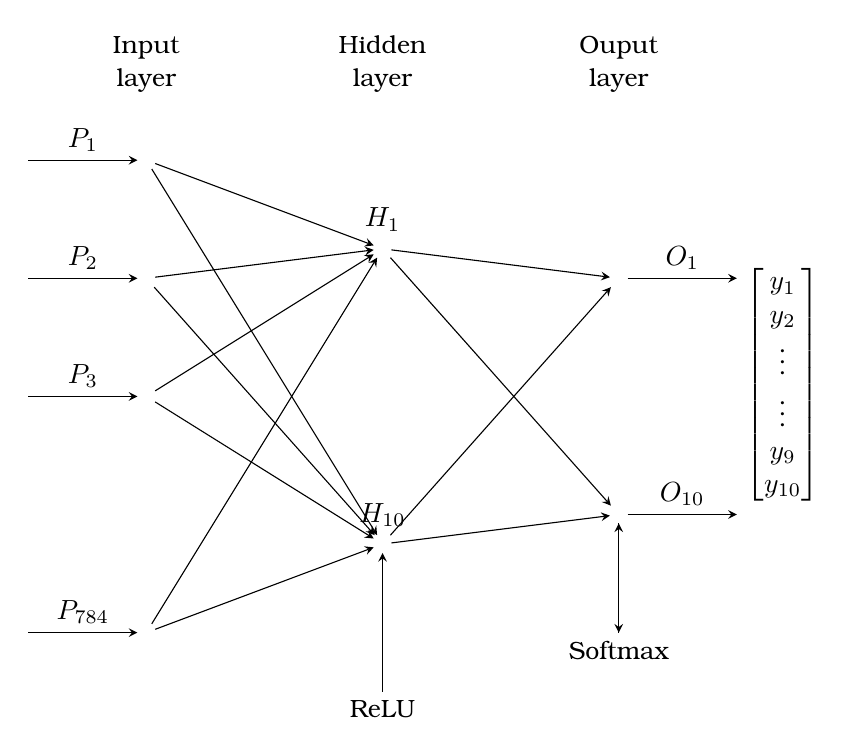
\begin{tikzpicture}[x=1.5cm, y=1.5cm, >=stealth]

\foreach \m/\l [count=\y] in {1,2,3,missing,4}
  \node [every neuron/.try, neuron \m/.try] (input-\m) at (0,2.5-\y) {};

\foreach \m [count=\y] in {1,missing,2}
  \node [every neuron/.try, neuron \m/.try ] (hidden-\m) at (2,2-\y*1.25) {};

\foreach \m [count=\y] in {1,missing,2}
  \node [every neuron/.try, neuron \m/.try ] (output-\m) at (4,1.5-\y) {};

\foreach \l [count=\i] in {1,2,3,784}
  \draw [<-] (input-\i) -- ++(-1,0)
    node [above, midway] {$P_{\l}$};

\foreach \l [count=\i] in {1,10}
  \node [above] at (hidden-\i.north) {$H_{\l}$};

\foreach \l [count=\i] in {1,10}
  \draw [->] (output-\i) -- ++(1,0)
    node [above, midway] {$O_{\l}$};

\foreach \i in {1,...,4}
  \foreach \j in {1,...,2}
    \draw [->] (input-\i) -- (hidden-\j);

\foreach \i in {1,...,2}
  \foreach \j in {1,...,2}
    \draw [->] (hidden-\i) -- (output-\j);

\foreach \l [count=\x from 0] in {Input, Hidden, Ouput}
  \node [align=center, above] at (\x*2,2) {\l \\ layer};


\node[anchor=west] at (5, -0.4) {$
    \begin{bmatrix}
        y_1 \\
        y_2 \\
        \vdots \\
        \vdots \\
        y_9 \\
        y_{10}
    \end{bmatrix}
$};


\draw[<-] (output-2) -- (4, -2.5) node[below] {Softmax};
\draw[->] (output-2) -- (4, -2.5);
\draw[<-] (hidden-2) -- (2, -3) node[below] {ReLU};


\end{tikzpicture}
\end{center}

Με $P_i\in \{1,2,\dots,255 \} $, $i= \{1,2, \dots , 784 \}$ να είναι η τιμή του i-οστού pixel, $H_i \ ,  \ i = \{1,2, \dots, 10 \}$ να είναι η τιμή του i-οστού νευρώνα στο hidden layer, $O_i \ , \ i = \{1,2,\dots,10 \}$ να είναι η τιμή του i-οστού νευρώνα στο outer layer πριν την εφαρμογή της softmax και τέλος $y_1, y_2, \dots , y_{10}$ να αποτελούν συνάρτηση πιθανότητας διακριτής κατανομής, δηλαδη $\sum_{i=1}^{10}y_i = 1$ και $y_i, i = \{1,2,\dots , 10 \}$, και το κάθε $y_i$ αντιστοιχεί στο $(i-1)$-αριθμό, $y_1 \to 0, y_2 \to 1 , \dots , y_{10} \to 9$ με $y_i$ η πιθανότητα το input να είναι το $(i-1)$-οστό νούμερο.

%%%%%%%%%%%%%%%%%%%%%%%%%%%%%%%%%%%%%%%%%%%%%%%%%%%%%%%%%%%%%%%%%%%%%%%%%%%%%%%%%%%%%%%%%%%%%%%%%%%%%%%%%%%%%%%%%%%%%%%%%%%%%%%%%%%%%%%%%%%%%%%%%%%%%%%%
%%%%%%%%%%%%%%%%%%%%%%%%%%%%%%%%%%%%%%%%%%%%%%%%%%%%%%%%%%%%%%%%%%%%%%%%%%%%
%%%%%%%%%%%%%%%%%%%%%%%%%%%%%%%%%%%%%%%%%%%%%%%%%%%%%%%%%%%%%%%%%%%%%%%%%%%%
%%%%%%%%%%%%%%%%%%%%%%%%%%%%%%%%%%%%%%%%%%%%%%%%%%%%%%%%%%%%%%%%%%%%%%%%%%%%
%%%%%%%%%%%%%%%%%%%%%%%%%%%%%%%%%%%%%%%%%%%%%%%%%%%%%%%%%%%%%%%%%%%%%%%%%%%%
%%%%%%%%%%%%%%%%%%%%%%%%%%%%%%%%%%%%%%%%%%%%%%%%%%%%%%%%%%%%%%%%%%%%%%%%%%%%

\newpage

\section*{}
\markright{Input}
\begin{center}
    \Large \textbf{Input}
\end{center}
\addcontentsline{toc}{section}{Input}



Το input αποτελέιται απο εικόνες διάστασης 28$\times$ 28 pixels (784 pixels στο σύνολο). Κάθε εικόνα μετατρέπεται σε ένα διάνυσμα διάστασης 784$\times$1. Επειδή οι τιμές κάθε pixels κυμάινονται απο το 0 μέχρι το 255, διαιρούμε κάθε τιμή του διανύσματος με 255 και κανονικοποιούμε κάθε τιμή στο διάστημα $[0,1]$

Επιπλέον αρχικοποιούμε τέσσερεις πίνακς έστω $W_1 \in \mathbb{M}^{784 \times 10}(\mathbb{R})$, $b_1 \in \mathbb{M}^{10 \times 1}(\mathbb{R})$, $W_2 \in \mathbb{M}^{10\times 10}(\mathbb{R})$ , $b_2 \in \mathbb{M}^{10 \times 1}(\mathbb{R})$ με $W_1$ να είναι τα βάρη που ενώνουν τις ακμές του input layer με το πρώτο, $b_1$ να είνα τα biases του πρώτου layer, $W_2$ τα βάρη που ενώνουν τις ακμές του πρώτου layer με το output layer και τέλος $b_1$ τα biases του output layer. 

%%%%%%%%%%%%%%%%%%%%%%%%%%%%%%%%%%%%%%%%%%%%%%%%%%%%%%%%%%%%%%%%%%%%%%%%%%%%%%%%%%%%%%%%%%%%%%%%%%%%%%%%%%%%%%%%%%%%%%%%%%%%%%%%%%%%%%%%%%%%%%%%%%%%%%%%
%%%%%%%%%%%%%%%%%%%%%%%%%%%%%%%%%%%%%%%%%%%%%%%%%%%%%%%%%%%%%%%%%%%%%%%%%%%%
%%%%%%%%%%%%%%%%%%%%%%%%%%%%%%%%%%%%%%%%%%%%%%%%%%%%%%%%%%%%%%%%%%%%%%%%%%%%
%%%%%%%%%%%%%%%%%%%%%%%%%%%%%%%%%%%%%%%%%%%%%%%%%%%%%%%%%%%%%%%%%%%%%%%%%%%%
%%%%%%%%%%%%%%%%%%%%%%%%%%%%%%%%%%%%%%%%%%%%%%%%%%%%%%%%%%%%%%%%%%%%%%%%%%%%


\newpage


\section*{}
\markright{ReLU, Softmax}
\begin{center}
    \Large \textbf{ReLU, Softmax (συναρτήσεις ενεργοποίησης)}
\end{center}
\addcontentsline{toc}{section}{ReLU, Softmax (συναρτήσεις ενεργοποίησης)}

\textbf{Ορισμός (ReLU):} Η συνάρτηση ReLU ορίζεται ως $φ: \mathbb{R} \to [0,\infty)$  
\[
φ(x) =
\begin{cases} 
x, & x \geq 0 \\
0, & x < 0
\end{cases}
\]

Η ReLU (και γενικότερα οι συναρτήσεις ενεργοποίσης) εισάγουν μη γραμμικότητα στο νευρωνικό μας δύκτιο. Ο υπολογισμός της τιμής ενός νευρώνα a, στο layer l, δίνεται ως ο γραμμικός συνδυασμός $a^{(l)} = Wa^{(l-1)} + b$. Επομένως χωρίς συνάρτηση ενεργοποίησης δεν θα είχε νόημα ο αριθμός των hidden layers και η γενικότερη πολυπλοκότητα του νευρωνικού δυκτίου καθώς το output θα ήταν πάλι μια γραμμική συνάρτηση.

$$$$

\textbf{Ορισμός (Softmax):} Η συνάρτηση Softmax, $σ: \mathbb{R}^n \to (0,1)^n , \ n>1$ για διάνυσμα $\mathbf{v} = (\mathrm{v}_1, \dots, \mathrm{v}_n) \in \mathbb{R}^n$ ορίζεται ως 
$$
σ(\mathbf{v}) = \big(σ(\mathrm{v}_1), \dots , σ(\mathrm{v}_n) \big)
$$
$$
\text{με} \ σ(\mathrm{v}_i) = \frac{e^{\mathrm{v}_i}}{\sum_{i=1}^n e^{\mathrm{v}_i}} 
$$

Η Softmax μετατρέπει το διάνυσμα $\mathrm{v}$ σε συνάρτηση πιθανότητας διακριτής κατανομής με $n$ ενδεχόμενα.

%%%%%%%%%%%%%%%%%%%%%%%%%%%%%%%%%%%%%%%%%%%%%%%%%%%%%%%%%%%%%%%%%%%%%%%%%%%%%%%%%%%%%%%%%%%%%%%%%%%%%%%%%%%%%%%%%%%%%%%%%%%%%%%%%%%%%%%%%%%%%%%%%%%%%%%%
%%%%%%%%%%%%%%%%%%%%%%%%%%%%%%%%%%%%%%%%%%%%%%%%%%%%%%%%%%%%%%%%%%%%%%%%%%%%
%%%%%%%%%%%%%%%%%%%%%%%%%%%%%%%%%%%%%%%%%%%%%%%%%%%%%%%%%%%%%%%%%%%%%%%%%%%%
%%%%%%%%%%%%%%%%%%%%%%%%%%%%%%%%%%%%%%%%%%%%%%%%%%%%%%%%%%%%%%%%%%%%%%%%%%%%
%%%%%%%%%%%%%%%%%%%%%%%%%%%%%%%%%%%%%%%%%%%%%%%%%%%%%%%%%%%%%%%%%%%%%%%%%%%%
%%%%%%%%%%%%%%%%%%%%%%%%%%%%%%%%%%%%%%%%%%%%%%%%%%%%%%%%%%%%%%%%%%%%%%%%%%%%
%%%%%%%%%%%%%%%%%%%%%%%%%%%%%%%%%%%%%%%%%%%%%%%%%%%%%%%%%%%%%%%%%%%%%%%%%%%%


\newpage

\section*{}
\markright{Mean squared error}
\begin{center}
    \Large \textbf{Mean squared error}
\end{center}
\addcontentsline{toc}{section}{Mean squared error}

Για τον υπολογισμό της απόκλισης του αποτελέσματος τους output layer απο το αναμενόμενο, έστω $μ$, θεωρούμε διάνυσμα $\mathbf{y} \in \mathbb{M}^{(n+1)\times 1}(\mathbb{R})$
\[
\mathbf{y} =  \begin{bmatrix}
    y_0 \\
    y_1 \\
    \vdots \\
    \vdots \\
    y_{n}
\end{bmatrix} \hspace{1cm} \text{με } 
\begin{cases} 
y_i = μ, & \text{αν } i = μ \\
0, & \text{διαφορετικά}
\end{cases}
\]

Έπειτα παίρνουμε το άθροισμα των τετραγώνων των διαφορών των τιμών του output με το $\mathbf{y}$. 

Αρα το loss του συστήματος, εξαρτάται απο το διάνυσμα που μας δίνει το output layer έπειτα απο την εφαρμογή της softmax αλλα και το $\mathbf{b}$, δηλαδή
\[
\mathcal{L}= \sum_{i=1}^{10} (a_i^{[L]} - y_i)^2 
\]

%%%%%%%%%%%%%%%%%%%%%%%%%%%%%%%%%%%%%%%%%%%%%%%%%%%%%%%%%%%%%%%%%%%%%%%%%%%%%%%%%%%%%%%%%%%%%%%%%%%%%%%%%%%%%%%%%%%%%%%%%%%%%%%%%%%%%%%%%%%%%%%%%%%%%%%%
%%%%%%%%%%%%%%%%%%%%%%%%%%%%%%%%%%%%%%%%%%%%%%%%%%%%%%%%%%%%%%%%%%%%%%%%%%%%
%%%%%%%%%%%%%%%%%%%%%%%%%%%%%%%%%%%%%%%%%%%%%%%%%%%%%%%%%%%%%%%%%%%%%%%%%%%%
%%%%%%%%%%%%%%%%%%%%%%%%%%%%%%%%%%%%%%%%%%%%%%%%%%%%%%%%%%%%%%%%%%%%%%%%%%%%
%%%%%%%%%%%%%%%%%%%%%%%%%%%%%%%%%%%%%%%%%%%%%%%%%%%%%%%%%%%%%%%%%%%%%%%%%%%%
%%%%%%%%%%%%%%%%%%%%%%%%%%%%%%%%%%%%%%%%%%%%%%%%%%%%%%%%%%%%%%%%%%%%%%%%%%%%
%%%%%%%%%%%%%%%%%%%%%%%%%%%%%%%%%%%%%%%%%%%%%%%%%%%%%%%%%%%%%%%%%%%%%%%%%%%%
%%%%%%%%%%%%%%%%%%%%%%%%%%%%%%%%%%%%%%%%%%%%%%%%%%%%%%%%%%%%%%%%%%%%%%%%%%%%
%%%%%%%%%%%%%%%%%%%%%%%%%%%%%%%%%%%%%%%%%%%%%%%%%%%%%%%%%%%%%%%%%%%%%%%%%%%%
%%%%%%%%%%%%%%%%%%%%%%%%%%%%%%%%%%%%%%%%%%%%%%%%%%%%%%%%%%%%%%%%%%%%%%%%%%%%



\newpage
\section*{}
\markright{Forward Propagation}
\begin{center}
    \Large \textbf{Forward Propagation}
\end{center}
\addcontentsline{toc}{section}{Forward Propagation} 

Όπως αναφέραμε και πιό πάνω, ο υπολογισμός της τιμής ενός νευρώνα $a_i$ στο layer l, δίνεται ως ο γραμμικός συνδυασμός 
\begin{equation}
a_{i}^{(l)} = w_{i,j} \cdot a_{j}^{(l-1)} + b_i \label{eq:linear}
\end{equation}
,  με $a_{j}^{(l-1)}$ ο j-νευρώνας στος layer $l-1$ , $w_{i,j}$ το βάρος της ακμής που συνδέει το i-νευρώνα με τον j-νευρώνα και $b_i$ το bias του i-νευρώνα. Επομένως αν θέλουμε να εκφράσουμε όλους του νευρώνες με την βοήθεια πινάκων θα έχουμε:

Για τις τιμές των νευρώνων στο hidden layer θα δείξουμε ότι ισχύει η ακόλουθη ισότητα
\begin{equation}
\mathbf{a^{(l)}} = W_{1}^{T} \mathbf{a^{(l-1)}} + \mathbf{b_1} \label{eq:forwardprop}
\end{equation}
με $W_{1}^{T}$ να είναι ο transpose πίνακας των βαρών μεταξύ input layer και hidden layer.

\begin{align}
\mathbf{a^{(l)}} &= W_{1}^{T} \mathbf{a^{(l-1)}} + \mathbf{b_1} \nonumber \\[10pt]
\Rightarrow \mathbf{a^{(1)}} &=  
\begin{bmatrix}
    w_{1,1} & w_{2,1} & \dots & w_{784,1} \\
    w_{1,2} & w_{2,2} & \dots & w_{784,2} \\
    \vdots & \vdots & \ddots & \vdots \\
    w_{1,10} & w_{2,10} & \dots & w_{784,10}
\end{bmatrix}
\begin{bmatrix}
    p_1 \\
    p_2 \\
    \vdots \\
    p_{784}
\end{bmatrix} + 
\begin{bmatrix}
    b_1 \\
    b_2 \\
    \vdots \\
    b_{10}
\end{bmatrix}  \nonumber \\[10pt]
\Rightarrow \mathbf{a^{(1)}} &= 
\begin{bmatrix}
   \sum_{i=1}^{784} w_{i,1} p_i + b_1 \\
   \sum_{i=1}^{784} w_{i,2} p_i + b_2 \\
   \vdots \\
   \sum_{i=1}^{784} w_{i,10} p_i + b_{10}
\end{bmatrix}, \quad \text{που είναι ακριβώς η εξίσωση~\eqref{eq:linear}, και άρα} \nonumber \\[10pt]
\Rightarrow \mathbf{a^{(1)}} &= 
\begin{bmatrix}
    a_{1}^{(l)} \\
    a_{2}^{(l)}  \\
    \vdots \\
    a_{10}^{(l)} 
\end{bmatrix} \nonumber
\end{align}


%%%%%%%%%%%%%%%%%%%%%%%%%%%%%%%%%%%%%%%%%%%%%%%%%%%%%%%%%%%%%%%%%%%%%%%%%%%%%%%%%%%%%%%%%%%%%%%%%%%%%%%%%%%%%%%%%%%%%%%%%%%%%%%%%%%%%%%%%%%%%%%%%%%%%%%%
%%%%%%%%%%%%%%%%%%%%%%%%%%%%%%%%%%%%%%%%%%%%%%%%%%%%%%%%%%%%%%%%%%%%%%%%%%%%
%%%%%%%%%%%%%%%%%%%%%%%%%%%%%%%%%%%%%%%%%%%%%%%%%%%%%%%%%%%%%%%%%%%%%%%%%%%%
%%%%%%%%%%%%%%%%%%%%%%%%%%%%%%%%%%%%%%%%%%%%%%%%%%%%%%%%%%%%%%%%%%%%%%%%%%%%
%%%%%%%%%%%%%%%%%%%%%%%%%%%%%%%%%%%%%%%%%%%%%%%%%%%%%%%%%%%%%%%%%%%%%%%%%%%%
%%%%%%%%%%%%%%%%%%%%%%%%%%%%%%%%%%%%%%%%%%%%%%%%%%%%%%%%%%%%%%%%%%%%%%%%%%%%
%%%%%%%%%%%%%%%%%%%%%%%%%%%%%%%%%%%%%%%%%%%%%%%%%%%%%%%%%%%%%%%%%%%%%%%%%%%%
%%%%%%%%%%%%%%%%%%%%%%%%%%%%%%%%%%%%%%%%%%%%%%%%%%%%%%%%%%%%%%%%%%%%%%%%%%%%
%%%%%%%%%%%%%%%%%%%%%%%%%%%%%%%%%%%%%%%%%%%%%%%%%%%%%%%%%%%%%%%%%%%%%%%%%%%%
%%%%%%%%%%%%%%%%%%%%%%%%%%%%%%%%%%%%%%%%%%%%%%%%%%%%%%%%%%%%%%%%%%%%%%%%%%%%



\newpage
\section*{}
\markright{Backward Propagation}
\begin{center}
    \Large \textbf{Backward Propagation}
\end{center}
\addcontentsline{toc}{section}{Backward Propagation} 

Ο στόχος μας είναι να ελαχιστοποιήσουμε το loss του νευρωνικού δυκτίου. Για να το πετύχουμε αυτό θα πρέπει αν βρούμε τα ελάχιστα της συνάρτησης του loss $\mathcal{L} = \sum_{i=1}^{10} (a_i^{(l)} - y_i)^2$. Για να βρούμε το ελάχιστό της ξεκινόντας απο ένα τυχαίο σημείο της, θα πρέπει να κινηθούμε προς την κατεύθυνση κατα την οποία η συνάρτηση μειώνεται γρηγορότερα.  Όμως απο θεωρία γνωρίζουμε οτι μια συνάρτηση $f$ αυξάνεται γρηγορότερα κατα την κατά την κατεύθυνση του διανύσματος $\overrightarrow{\nabla f}$ και επομένως θα πρέπει να κινηθούμε στην κατεύθυνση του διανύσματος $-\overrightarrow{\nabla f}$. 

Άρα για την συνάρητηση $\mathcal{L}$ αρκεί να βρούμε την παράγωγό της προς όλα τα βάρη και biases δηλαδη για τα βάρη στο $l$-layer

$$
\frac{\partial \mathcal{L}}{\partial w_{i}^{(l)}}  \    \text{και} \  \frac{\partial \mathcal{L}}{\partial b_{j}^{(l)}}
\ , \ \forall i , \forall j
$$
Επομένως μέχρι τώρα έχουμε
\[
z_{i}^{(l)} = w_{i,j}^{(l)} \cdot a_{j}^{(l-1)} + b_{i}^{(l)}
\]
η τιμή του νευρώνα i πριν εφαρμόσουμε την συνάρτηση ενεργοποίησης.

Έστω σ η συνάρτηση ενεργοποίησης και $a_i$ η τιμή του νευρώνα μετα την εφαρμογή της σ, δηλαδή
\[
a_{i}^{(l)} = σ(z_{i}^{(l)})
\]
Άρα απο τον κανόνα της αλυσίδας έχουμε για τα βάρη που συνδέουν το hidden με το output layer

\begin{align}
\frac{\partial \mathcal{L}}{\partial w_{i}^{(l)}}  &= \frac{\partial \mathcal{L}}{\partial a_{i}^{(l)}}  \cdot \frac{\partial a_{i}^{(l)}}{\partial z_{i}^{(l)}}  \cdot \frac{\partial z_{i}^{(l)}}{\partial w_{i,j}^{(l)}} \label{eq:grad_weight_l1} \\
\Rightarrow \frac{\partial \mathcal{L}}{\partial w_{i}^{(l)}} &= 2(a_i^{(l)} - y_{i}) \cdot \mathbf{1}_{\{z_{i}^{(l)}>0\} } \cdot a_{j}^{(l-1)} \label{eq:grad_weight_l2}
\end{align}

Αντίστοιχα για τα biases

\begin{align}
\frac{\partial \mathcal{L}}{\partial b_{i}^{(l)}}  &= \frac{\partial \mathcal{L}}{\partial a_{i}^{(l)}}  \cdot \frac{\partial a_{i}^{(l)}}{\partial z_{i}^{(l)}}  \cdot \frac{\partial z_{i}^{(l)}}{\partial b_{i}^{(l)}} \label{eq:grad_bias_l1} \\
\Rightarrow \frac{\partial \mathcal{L}}{\partial b_{i}^{(l)}} &= 2(a_i^{(l)} - y_{i}) \cdot \mathbf{1}_{\{z_{i}^{(l)}>0\} } \cdot 1 \label{eq:grad_bias_l2}
\end{align}

\newpage

Όμως τα πράγματα δυσκολεύουν όταν πάμε να υπολογίσουμε τις ίδες παραγώγους για τα βάρη και τα biases μεταξύ input και hidden layer.

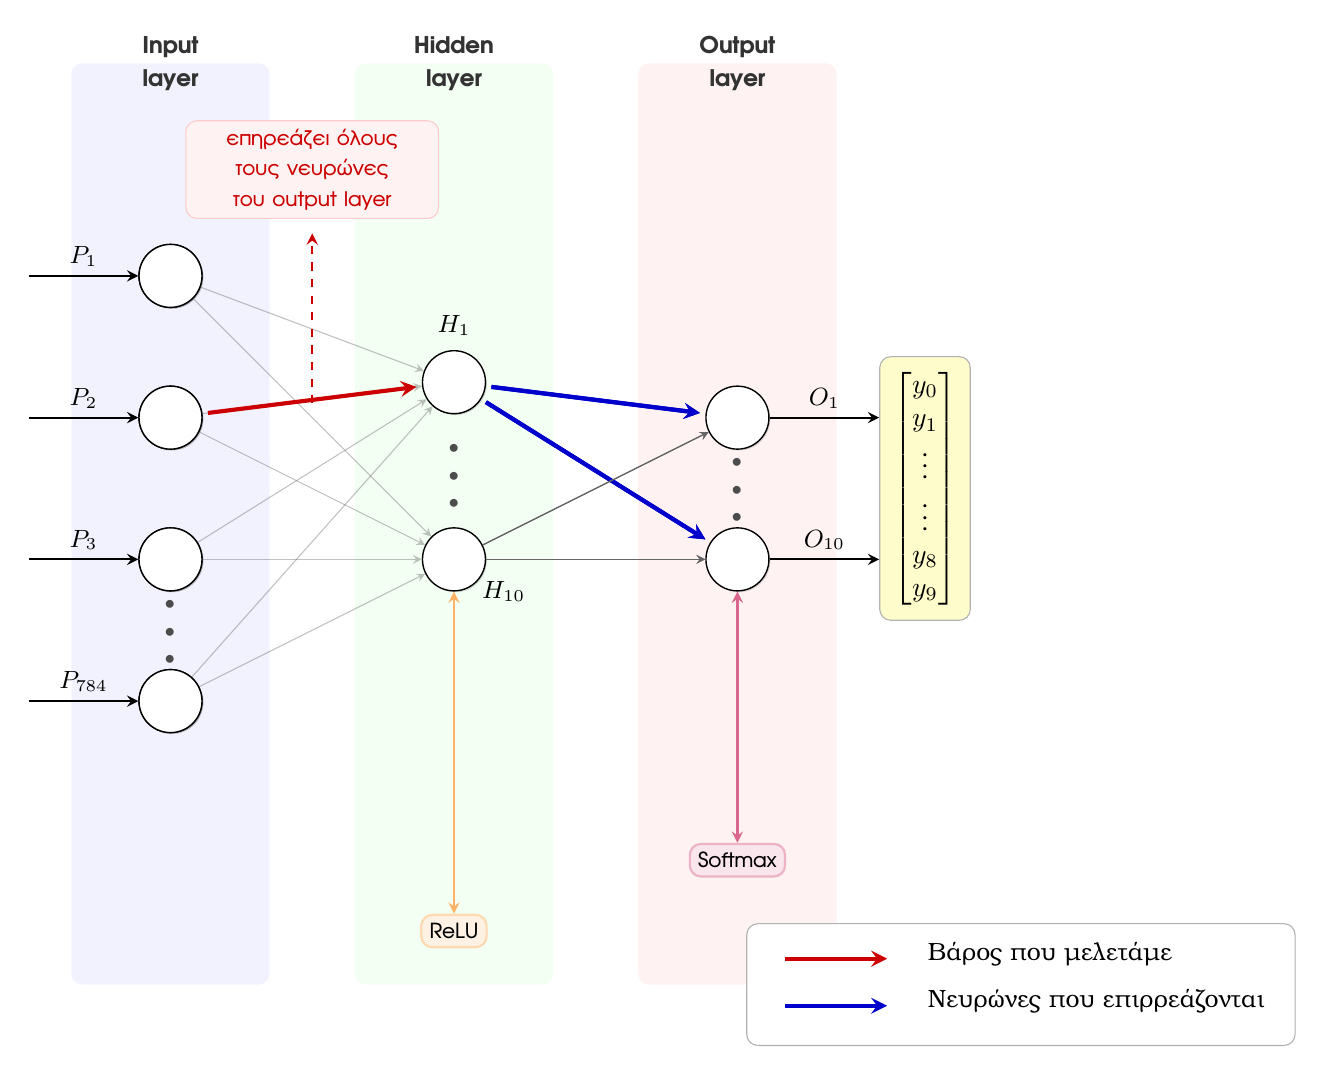
\begin{tikzpicture}[
    x=1.8cm, y=1.8cm, >=stealth,
    % Improved neuron styles
    neuron/.style={
        circle, 
        draw=black, 
        fill=white, 
        line width=0.5pt,
        minimum size=0.8cm,
        drop shadow={shadow xshift=0.5pt, shadow yshift=-0.5pt, opacity=0.3}
    },
    neuron missing/.style={
        draw=none, 
        scale=2.5, 
        text height=0.333cm, 
        execute at begin node=\color{black!70}
    },
    % Improved edge styles
    regular edge/.style={->, draw=black!60, thin},
    bold input edge/.style={
        ->, 
        draw=red!80!black, 
        line width=1.5pt,
        shorten >=2pt,
        shorten <=2pt
    },
    bold output edge/.style={
        ->, 
        draw=blue!80!black, 
        line width=1.5pt,
        shorten >=2pt,
        shorten <=2pt
    },
    % Label styles
    layer label/.style={
        align=center, 
        font=\sffamily\bfseries, 
        text=black!80
    },
    neuron label/.style={
        font=\sffamily\small
    }
]

% Background shading for layers
\begin{scope}[on background layer]
    \fill[blue!5, rounded corners] (-0.7,3) rectangle (0.7,-3.5);
    \fill[green!5, rounded corners] (1.3,3) rectangle (2.7,-3.5);
    \fill[red!5, rounded corners] (3.3,3) rectangle (4.7,-3.5);
\end{scope}

% -------------------------------
% Επίπεδο εισόδου (input layer)
\foreach \i [count=\y] in {1,2,3,4}
{
    \node[neuron] (input-\i) at (0,2.5-\y) {};
}
% Κόμβος έλλειψης (missing) στο input layer
\foreach \i [count=\y] in {1,2,3,4}
{
    \node[neuron] (input-\i) at (0,2.5-\y) {};
}
\node[neuron missing] (input-missing) at (0, -1) {$\vdots$};

% -------------------------------
% Κρυφό επίπεδο (hidden layer)
\foreach \i [count=\y] in {1,2}
{
    \node[neuron] (hidden-\i) at (2,2-\y*1.25) {};
}
\node[neuron missing] (hidden-missing) at (2, 0.1) {$\vdots$};

% -------------------------------
% Επίπεδο εξόδου (output layer)
\foreach \i [count=\y] in {1,2}
{
    \node[neuron] (output-\i) at (4,1.5-\y) {};
}
\node[neuron missing] (output-missing) at (4,  0) {$\vdots$};

% -------------------------------
% Ετικέτες εισόδου
\foreach \i/\lbl in {1/1, 2/2, 3/3, 4/784}
    \draw[<-, thick] (input-\i) -- ++(-1,0) 
        node[above, midway, neuron label] {$P_{\lbl}$};

% Ετικέτες κρυφού επιπέδου
\foreach \i/\lbl in {1/1}
    \node[above=2pt, neuron label] at (hidden-\i.north) {$H_{\lbl}$};
\foreach \i/\lbl in {2/10}
    \node[right=7pt, neuron label] at (hidden-\i.south) {$H_{\lbl}$};

% Ετικέτες εξόδου
\foreach \i/\lbl in {1/1, 2/10}
    \draw[->, thick] (output-\i) -- ++(1,0) 
        node[above, midway, neuron label] {$O_{\lbl}$};

% -------------------------------
% Ακμές από input σε hidden με διαφάνεια για καλύτερη αναγνωσιμότητα
\foreach \i in {1,2,3,4}
    \foreach \j in {1,2}
    {
        \draw[regular edge, opacity=0.4] (input-\i) -- (hidden-\j);
    }

% Τονισμένη ακμή από input-2 σε hidden-1 (πάνω από τις άλλες για ορατότητα)
\draw[bold input edge] (input-2) -- (hidden-1);

% -------------------------------
% Ακμές από hidden σε output (τονισμένες)
\foreach \i in {1,1}
    \foreach \j in {1,2}
    {
        \draw[bold output edge] (hidden-\i) -- (output-\j);
    }
\foreach \i in {2,2}
    \foreach \j in {2,1}
    {
        \draw[regular edge] (hidden-\i) -- (output-\j);
    }

% -------------------------------
% Επικεφαλίδες επιπέδων με βελτιωμένο στυλ
\node[layer label] at (0,3) {Input\\layer};
\node[layer label] at (2,3) {Hidden\\layer};
\node[layer label] at (4,3) {Output\\layer};

% -------------------------------
% Διάνυσμα εξόδου με πλαίσιο
\node[anchor=west, draw=black!30, rounded corners, fill=yellow!20, inner sep=5pt] at (5, 0) {$
    \begin{bmatrix}
        y_0 \\
        y_1 \\
        \vdots \\
        \vdots \\
        y_8 \\
        y_{9}
    \end{bmatrix}
$};

% -------------------------------
% Συναρτήσεις ενεργοποίησης με καλύτερο στυλ
\draw[<->, thick, draw=purple!60] (output-2) -- (4, -2.5) 
    node[below, rounded corners, fill=purple!10, draw=purple!30, 
         inner sep=3pt, font=\sffamily\small] {Softmax};
\draw[<->, thick, draw=orange!60] (hidden-2) -- (2, -3) 
    node[below, rounded corners, fill=orange!10, draw=orange!30, 
         inner sep=3pt, font=\sffamily\small] {ReLU};

% -------------------------------
% Επεξήγηση τονισμένης ακμής input-hidden
\node[
    text width=3cm, 
    align=center, 
    font=\small\sffamily, 
    color=red!80!black,
    fill=red!5,
    rounded corners,
    draw=red!20,
    inner sep=3pt
] at (1, 2.25) {επηρεάζει όλους τους νευρώνες του output layer};
\draw[->, red!80!black, dashed, thick] (1, 0.6) -- (1, 1.8);

% -------------------------------
% Υπόμνημα σε πλαίσιο
\node[draw=black!30, fill=white, rounded corners, inner sep=5pt] at (6, -3.5) {
    \begin{tabular}{l l}
        \tikz \draw[bold input edge] (0,0) -- (0.8,0); & Βάρος που μελετάμε  \\[5pt]
        \tikz \draw[bold output edge] (0,0) -- (0.8,0); & Νευρώνες που επιρρεάζονται  \\[5pt]
    \end{tabular}
};

% Κείμενο τίτλου
\end{tikzpicture}

Στην περίπτωση αυτή κάθε βάρος και bias συμβάλει στο διάνυσμα του output layer και επομένως η μερική παράγωγος του loss προς αυτά θα είναι πιο σύνθετη. Συγκεκριμένα για τα βαρη και biases του $l-1$ layer θα έχουμε

\begin{align}
\frac{\partial \mathcal{L}}{\partial w_{i}^{(l-1)}}  &=  \frac{\partial a_{i}^{(l-1)}}{\partial z_{i}^{(l-1)}}  \cdot \frac{\partial z_{i}^{(l-1)}}{\partial w_{i,j}^{(l-1)}} \cdot \frac{\partial \mathcal{L}}{\partial a_{i}^{(l-1)}}  \label{eq:grad_weight1} \\
\Rightarrow \frac{\partial \mathcal{L}}{\partial w_{i}^{(l-1)}}  &= \mathbf{1}_{\{z_{i}^{(l-1)}>0\} } \cdot a_{i}^{(l-2)} \cdot \sum_{i} w_{k,i}^{(l)}\mathbf{1}_{\{z_{i}^{(l)}>0\} } 2(a_{i}^{(l)} - y_i) \label{eq:grad_weight2}
\end{align}

Αντίστοιχα για τα biases έχουμε 

\begin{align}
\frac{\partial \mathcal{L}}{\partial b_{i}^{(l-1)}}  &= \frac{\partial a_{i}^{(l-1)}}{\partial z_{i}^{(l-1)}}  \cdot \frac{\partial z_{i}^{(l-1)}}{\partial b_{i}^{(l-1)}} \cdot \frac{\partial \mathcal{L}}{\partial a_{i}^{(l-1)}} \label{eq:grad_bias1} \\
\Rightarrow \frac{\partial \mathcal{L}}{\partial b_{i}^{(l-1)}}  &= \mathbf{1}_{\{z_{i}^{(l-1)}>0\} } \cdot 1 \cdot \sum_{i} w_{k,i}^{(l)}\mathbf{1}_{\{z_{i}^{(l)}>0\} } 2(a_{i}^{(l)} - y_i) \label{eq:grad_bias2}
\end{align}


Επομένως για να υπολογίσουμε τις παραγώγους όλων των βαρών και biases με την βοήθεια πινάκων, θα δείξουμε ότι 
\begin{align*}
\frac{\partial \mathcal{L}}{\partial w_{i}^{(2)}}  &= \mathbf{a}^{(1)} [2(\mathbf{a}^{(2)} - \mathbf{y})]^{T} \\
\Rightarrow \frac{\partial \mathcal{L}}{\partial w_{i}^{(2)}}  &= 
\begin{bmatrix}
    a_{1}^{(1)} \\
    a_{2}^{(1)}  \\
    \vdots \\
    a_{10}^{(1)} 
\end{bmatrix} 
\begin{bmatrix}
    2(a_{1}^{(2)} - y_1) &  2(a_{2}^{(2)} - y_2)  & \cdots & 2(a_{10}^{(2)} - y_{10}) 
\end{bmatrix} \\
\Rightarrow \frac{\partial \mathcal{L}}{\partial w_{i}^{(2)}}  &= 
\begin{bmatrix}
a_{1}^{(1)} \cdot 2(a_{1}^{(2)} - y_1) & a_{1}^{(1)} \cdot 2(a_{2}^{(2)} - y_2) & \cdots & a_{1}^{(1)} \cdot 2(a_{10}^{(2)} - y_{10}) \\
\vdots & \vdots & \ddots & \vdots \\
\vdots & \vdots &  & \vdots \\
a_{10}^{(1)} \cdot 2(a_{1}^{(2)} - y_1) & a_{10}^{(1)} \cdot 2(a_{2}^{(2)} - y_2) & \cdots & a_{10}^{(1)} \cdot 2(a_{10}^{(2)} - y_{10})
\end{bmatrix} 
\end{align*}
Επομένως κάθε στοιχείο του πίνακα είναι της μορφής 
$
2(a_i^{(l)} - y_{i}) \cdot  a_{j}^{(l-1)}  , \forall i,j \in \{1,2, \dots ,10 \}
$
και άρα 
\[
 \frac{\partial \mathcal{L}}{\partial w_{i}^{(2)}}  = 
 \begin{bmatrix}
    \frac{\partial \mathcal{L}}{\partial w_{1}^{(2)}}  \\
    \frac{\partial \mathcal{L}}{\partial w_{2}^{(2)}}  \\
    \vdots \\
    \frac{\partial \mathcal{L}}{\partial w_{10}^{(2)}}
\end{bmatrix}  \quad \text{(χρισημοποιώντας την \(\eqref{eq:grad_weight_l2}\))}
\]
το οποίο είναι τετριμμένο.
\\
Επίσης θα δείξουμε ότι 
\begin{align*}
\frac{\partial \mathcal{L}}{\partial b_{i}^{(2)}}  &= 2(\mathbf{a}^{(2)} - \mathbf{y}) \\
\Rightarrow \frac{\partial \mathcal{L}}{\partial b_{i}^{(2)}}  &= 
\begin{bmatrix}
    2(a_{1}^{(2)} - y_1) \\
     2(a_{2}^{(2)} - y_2)  \\
      \vdots \\ 
       2(a_{10}^{(2)} - y_{10}) 
\end{bmatrix}  \\
\Rightarrow \frac{\partial \mathcal{L}}{\partial b_{i}^{(2)}}  &= 
\begin{bmatrix}
\frac{\partial \mathcal{L}}{\partial b_{1}^{(2)}} \\
\frac{\partial \mathcal{L}}{\partial b_{2}^{(2)}} \\
\vdots \\
\frac{\partial \mathcal{L}}{\partial b_{10}^{(2)}}
\end{bmatrix} \quad \text{(χρισημοποιώντας την \(\eqref{eq:grad_bias_l2}\))}
\end{align*}
επίσης τετριμμένο αποτέλεσμα.
\\
Θα δείξουμε ότι 
\begin{align*}
\frac{\partial \mathcal{L}}{\partial w_{i}^{(2)}}  &= \mathbf{a}^{(0)} \big [ \mathbf{w^{(2)}} [2(\mathbf{a}^{(2)} - \mathbf{y})] \big ]^{T} \\
\Rightarrow \frac{\partial \mathcal{L}}{\partial w_{i}^{(2)}}  &= 
\begin{bmatrix}
    p_1 \\
    p_2 \\
    \vdots \\
    p_{784}
\end{bmatrix}
\left[
\begin{bmatrix}
w_{1,1} & w_{1,2} & \ldots & w_{1,10} \\
w_{2,1} & w_{2,2} & \ldots & w_{2,10} \\
\vdots & \vdots & \ddots & \vdots \\
w_{10,1} & w_{10,2} & \ldots & w_{10,10}
\end{bmatrix}
\begin{bmatrix}
    2(a_{1}^{(2)} - y_1) \\
     2(a_{2}^{(2)} - y_2)  \\
      \vdots \\ 
       2(a_{10}^{(2)} - y_{10}) 
\end{bmatrix}
\right] ^{T} \\
\Rightarrow  \frac{\partial \mathcal{L}}{\partial w_{i}^{(2)}}  &= 
\begin{bmatrix}
    p_1 \\
    p_2 \\
    \vdots \\
    p_{784}
\end{bmatrix}
\begin{bmatrix}
    w_{1,1} \cdot 2(a_{1}^{(2)} - y_1) + w_{1,2} \cdot 2(a_{2}^{(2)} - y_2) + \ldots + w_{1,10} \cdot 2(a_{10}^{(2)} - y_{10}) \\
    w_{2,1} \cdot 2(a_{1}^{(2)} - y_1) + w_{2,2} \cdot 2(a_{2}^{(2)} - y_2) + \ldots + w_{2,10} \cdot 2(a_{10}^{(2)} - y_{10}) \\
    \vdots \\
    w_{10,1} \cdot 2(a_{1}^{(2)} - y_1) + w_{10,2} \cdot 2(a_{2}^{(2)} - y_2) + \ldots + w_{10,10} \cdot 2(a_{10}^{(2)} - y_{10})
\end{bmatrix} ^{T} \\
\Rightarrow  \frac{\partial \mathcal{L}}{\partial w_{i}^{(2)}}  &= 
\begin{bmatrix}
    p_1 \\
    p_2 \\
    \vdots \\
    p_{784}
\end{bmatrix}
\begin{bmatrix}
    \sum_{j=1}^{10} w_{1,j} \cdot 2(a_{j}^{(2)} - y_j) \\
    \sum_{j=1}^{10} w_{2,j} \cdot 2(a_{j}^{(2)} - y_j) \\
    \vdots \\
    \sum_{j=1}^{10} w_{10,j} \cdot 2(a_{j}^{(2)} - y_j)
\end{bmatrix} ^ {T} \\
\Rightarrow  \frac{\partial \mathcal{L}}{\partial w_{i}^{(2)}}  &= 
\begin{bmatrix}
    p_1 \\
    p_2 \\
    \vdots \\
    p_{784}
\end{bmatrix}
\begin{bmatrix}
    \sum_{j=1}^{10} w_{1,j} \cdot 2(a_{j}^{(2)} - y_j) & 
    \cdots & 
    \sum_{j=1}^{10} w_{10,j} \cdot 2(a_{j}^{(2)} - y_j)
\end{bmatrix} \\
\Rightarrow  \frac{\partial \mathcal{L}}{\partial w_{i}^{(2)}}  &= 
\begin{bmatrix}
    p_1 \sum_{j=1}^{10} w_{1,j} \cdot 2(a_{j}^{(2)} - y_j) & \cdots & p_1 \sum_{j=1}^{10} w_{10,j} \cdot 2(a_{j}^{(2)} - y_j) \\
    \vdots & \ddots & \vdots \\
    p_{784} \sum_{j=1}^{10} w_{1,j} \cdot 2(a_{j}^{(2)} - y_j) & \cdots & p_{784} \sum_{j=1}^{10} w_{10,j} \cdot 2(a_{j}^{(2)} - y_j)
\end{bmatrix} \\
\Rightarrow  \frac{\partial \mathcal{L}}{\partial w_{i}^{(2)}}  &= 
\begin{bmatrix}
    \frac{\partial \mathcal{L}}{\partial w_{1,1}^{(2)}} & \frac{\partial \mathcal{L}}{\partial w_{1,2}^{(2)}} & \cdots & \frac{\partial \mathcal{L}}{\partial w_{1,10}^{(2)}} \\
    \frac{\partial \mathcal{L}}{\partial w_{2,1}^{(2)}} & \frac{\partial \mathcal{L}}{\partial w_{2,2}^{(2)}} & \cdots & \frac{\partial \mathcal{L}}{\partial w_{2,10}^{(2)}} \\
    \vdots & \vdots & \ddots & \vdots \\
    \frac{\partial \mathcal{L}}{\partial w_{784,1}^{(2)}} & \frac{\partial \mathcal{L}}{\partial w_{784,2}^{(2)}} & \cdots & \frac{\partial \mathcal{L}}{\partial w_{784,10}^{(2)}}
\end{bmatrix} \quad \text{(χρισημοποιώντας την \(\eqref{eq:grad_weight2}\))}
\end{align*}


%%%%%%%%%%%%%%%%%%%%%%%%%%%%%%%%%%%%%%%%%%%%%%%%%%%%%%%%%%%%%%%%%%%%%%%%%%%%%%%%%%%%%%%%%%%%%%%%%%%%%%%%%%%%%%%%%%%%%%%%%%%%%%%%%%%%%%%%%%%%%%%%%%%%%%%%
%%%%%%%%%%%%%%%%%%%%%%%%%%%%%%%%%%%%%%%%%%%%%%%%%%%%%%%%%%%%%%%%%%%%%%%%%%%%
%%%%%%%%%%%%%%%%%%%%%%%%%%%%%%%%%%%%%%%%%%%%%%%%%%%%%%%%%%%%%%%%%%%%%%%%%%%%
%%%%%%%%%%%%%%%%%%%%%%%%%%%%%%%%%%%%%%%%%%%%%%%%%%%%%%%%%%%%%%%%%%%%%%%%%%%%
%%%%%%%%%%%%%%%%%%%%%%%%%%%%%%%%%%%%%%%%%%%%%%%%%%%%%%%%%%%%%%%%%%%%%%%%%%%%
%%%%%%%%%%%%%%%%%%%%%%%%%%%%%%%%%%%%%%%%%%%%%%%%%%%%%%%%%%%%%%%%%%%%%%%%%%%%
%%%%%%%%%%%%%%%%%%%%%%%%%%%%%%%%%%%%%%%%%%%%%%%%%%%%%%%%%%%%%%%%%%%%%%%%%%%%
%%%%%%%%%%%%%%%%%%%%%%%%%%%%%%%%%%%%%%%%%%%%%%%%%%%%%%%%%%%%%%%%%%%%%%%%%%%%
%%%%%%%%%%%%%%%%%%%%%%%%%%%%%%%%%%%%%%%%%%%%%%%%%%%%%%%%%%%%%%%%%%%%%%%%%%%%
%%%%%%%%%%%%%%%%%%%%%%%%%%%%%%%%%%%%%%%%%%%%%%%%%%%%%%%%%%%%%%%%%%%%%%%%%%%%



\newpage
\section*{}
\markright{Gradient Descent}
\begin{center}
    \Large \textbf{Gradient Descent}
\end{center}
\addcontentsline{toc}{section}{Gradient Descent} 

Όπως αναφέραμε και στο Back propagation, στόχος μας είναι να βρούμε το ολικό ελάχιστο της συνάρτησης κόστους  $\mathcal{L}$ και άρα να κινηθούμε στην κατεύθυνση του $\overrightarrow{\nabla f}$
Γράφω κάτι όχι συγκεκριμένο και καινούριο $$\sum_{min}^{max} \mathcal{X}$$

\end{document}